%%%%%%%%%%%%%%%%%%%%%%%%%%%%%%%%%%%%%%%%%
% University/School Laboratory Report
% LaTeX Template
% Version 2.0 (4/12/12)
%
% This template has been downloaded from:
% http://www.latextemplates.com
%
% License:
% CC BY-NC-SA 3.0 (http://creativecommons.org/licenses/by-nc-sa/3.0/)
%
% Original header:
%
%
%%%%%%%%%%%%%%%%%%%%%%%%%%%%%%%%%%%%%%%%%

%----------------------------------------------------------------------------------------
%	DOCUMENT CONFIGURATIONS
%----------------------------------------------------------------------------------------

\documentclass{article}

\usepackage{graphicx} % Allows the inclusion of images

\title{Writing Customable Cython Neurons \\ Developer Documentation} % Title

\author{Jonny \textsc{Quarta}} % Author name

\date{\today} % Specify a date for the report

\begin{document}

\maketitle % Insert the title, author and date


\setlength\parindent{0pt} % Removes all indentation from paragraphs

\renewcommand{\labelenumi}{\alph{enumi}.} % Make numbering in the enumerate environment by letter rather than number (e.g. section 6)

\section{Introduction}
The NEST Simulator, which stands for Neural Simulation Tool, has been created with the purpose of enabling complex simulations of point-like neurons. There's a wide range of possible models, from the simple integrate and fire model, to the more complex Hodgkin-Huxley one.\\
These neurons can be connected throught weighted connexions and their activity recorded using virtual tools (multimeter, spike detector, etc...).\\

In the NEST code, every model extends from a parent class, implementing only basic functions, such as collecting the incoming spikes. The real model is written in the child classes, so that, using polymorphism, adding new neurons is accomplished relatively easily.\\
However, each time one wants to add a new neuron, he has to write it in C++ (a difficult language) and recompile the whole project. This makes the tool not so flexible and slows down developpement time.\\
That's why the need for a plugin system has arised. Since NEST provides an interface enabling the user to execute the simulator from a PYthon terminal, the system has to be designed in order to facilitate the python utilization.
Therefore, this new feature should enable to easily write neurons and import them like normal python objects, these being automatically recognized and executed by NEST like normal neurons. In addition, since C++ is a difficult language, models should be written in a more scientific language such as Cython.\\ \\
The purpose of this project is the creation of a plugin system having these features. This is accomplished using a relatively new technology, Cython. This special tool enables one to write Python code and compile it into C++ or writing cython code and interface it with Python.\\
During the next sections, first the NEST structure will be presented, then a global description of the interface will be depicted. After that, more details are given, beginning with the NEST C++ side, followed by the CyNEST (the Cython) side. Finally, performances and improvements are analyzed.

\section{NEST Structure}
The aim of this section is to enable the reader understanding the global NEST structure, which is essential in order to grasp the details of the new interface, presented in the next sections.\\
Basically, NEST is composed of three major parts:
\begin{itemize}
\item The simulation kernel : this is the core of the system, enabling, among others, simulations, events scheduling, communication of neurons and activity recording. The C++ models are also situated in this part.
\item SLI Interface : NEST is a high configurable simulator, therefore a powerfull language has been created in order to configure simulation properties, set experiment parameters, create neurons and connexions between them, ect... SLI is loosely based on PostScript, using a stack to put, manipulate and retrieve objects.
\item CyNEST Interface : NEST can be used from a Python terminal, configuring it by calling very high functions, which will in turn call corresponding SLI commands. This interface can be accessed by just typing \emph{import cynest} in a Python terminal.
\end{itemize}
For more information, see the original documentation\\ (http://www.nest-initiative.org/index.php/Software:About\_NEST).

\section{Global Interface Structure}
This section deals with the global structure of the new interface between NEST and custom neurons. 

\begin{figure}[h]
\begin{center}
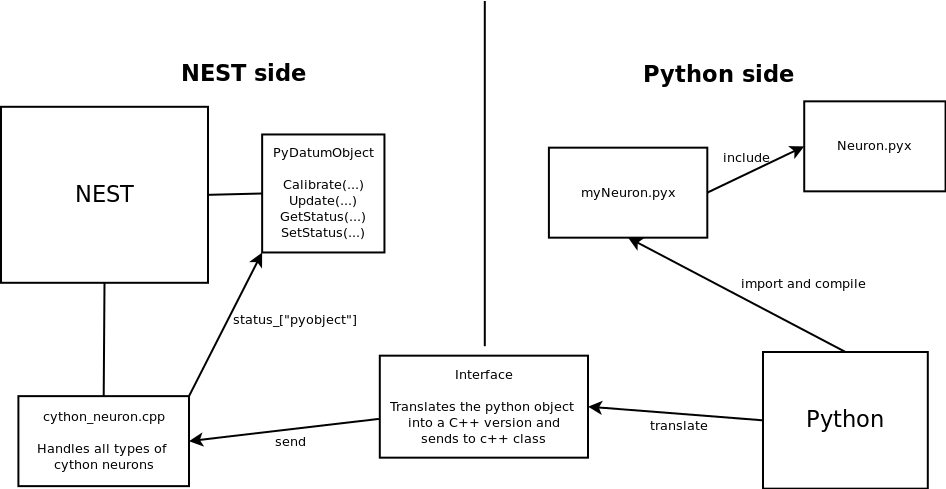
\includegraphics[width=0.92\textwidth]{Ressources/Interface_Structure}
\caption{Interface Structure}
\end{center}
\end{figure}

Figure 1 shows that structure as a diagram. The key idea is quite simple: the user writes his models as .pyx files and imports them into CyNEST via the python terminal. Then, whenever he creates a new instance of a custom neuron, CyNEST will transform it into a C++ version and give it to the \emph{cython\_neuron.cpp} class, which will then call the corresponding methods (update, calibrate, etc...). Therefore, the C++ side will use the C/Python API in order to access the python object fields and methods.\\

During the next sections, the most important regions of the diagram will be covered in much greater detail, so that the reader can have insight into the subtle choises and concepts that populate this innovative feature of NEST.



\section{Python Side}
This section focuses on the main operations the Python side has to accomplish in order to make the system work.\\

\subsection{Base Neuron Class}
First of all, the model has to be written (for details about how to wrtite new models, please consult the user documentation).\\
However, it is important to know what structure the model relies on. This is the base, called \emph{Neuron} and located in the \emph{"installation folder"/include/Neuron.pyx} file, with the installation path being where CyNEST has been installed. This file contains the following code:
\begin{verbatim}
cdef class Neuron:
    cdef object time_scheduler
    # Standard Parameters
    cdef double currents
    ...
    
    def __cinit__(self):
        pass

    cpdef calibrate(self):
        pass
        
    cpdef update(self):
        pass
        
    ...
        
    cpdef setTimeScheduler(self, ts):
        self.time_scheduler = ts
       
    # We convert the address of the variables into long in order to extract the pointers

    cpdef getPCurrents(self):
        return <long>(&(self.currents))
        
    ...
\end{verbatim}
Note that not everything is shown.\\
The class is composed of various parameters, whose usefullness will be discussed later, and  other functions, some of which have to be overwritten by the child model. These functions are \emph{calibrate}, \emph{update}, \emph{setStatus} and \emph{getStatus}. The other functions will be explained during the next sections.


\subsection{Neuron Registration}
Once the model has been completed, the user has to load it before any utilization. This process is called \textbf{neuron registration}.\\
Indeed, the first thing to do is typing \emph{cynest.RegisterNeuron(...)}. This method will use a cython mechanism, called \textbf{pyximport}, to dinamically import and compile the .pyx file containing the custom model:
\begin{verbatim}
def RegisterNeuron(model_name):
    exec("import " + model_name)
    globals()[model_name] = locals()[model_name]
    cython_models.append(model_name)
    reg(model_name)
\end{verbatim}
Here we can see that the model is compiled and imported. \emph{cython\_models} is a list containing the name of the custm models, used when the software has to check if a neuron is normal or custom. The final step is to actually register the model into the system and is accomplished by the \emph{reg} function, which actually corresponds to the \emph{register\_cython\_model} method contained in the \emph{cynest/cynestkernel.cpp} file.\\

When a new model instance is created, NEST will search that particular model among its classes. But how to know if a model has a corresponding class (i.e., if it exists)? The \emph{models/modelsmodule.cpp} class provides the answer. Every new model is registered in the \textbf{models dictionary}, so that when a new instance has to be created, NEST just checks in this dictionary, looks for that particular model and creates the corresponding class object.\\
In order to register a new model, a code such this has to be written :
\begin{verbatim}
	register_model<iaf_cond_alpha>(net_, "iaf_cond_alpha");
\end{verbatim}
Here, the first \emph{iaf\_cond\_alpha} corresponds to the class name, whereas the second one corresponds to the string pointing to that particular class.\\
Therefore, the \emph{register\_cython\_model} method finally calls a statement like this:
\begin{verbatim}
	register_model<cython_neuron>(net_, model_name);
\end{verbatim}
For more information, look to the \emph{models/modelsmodule.cpp} file.

\subsection{Neuron Creation}
After a neuron is registered, new instances are created with the \emph{cynest.Create(..)} method.
Here, the main task is to check whether the neuron is a normal or a custom one, as well as sending the model to the c++ class if it is the case:
\begin{verbatim}
if model in cython_models:
    for i in ids:
        exec("tmpobj___ = " + model + "." + model + "()")
        tmpobj___.setTimeScheduler(t_sched)
        SetStatus([i], {'pyobject':tmpobj___})
\end{verbatim}
The function actually creates an intermediate object corresponding to the custom model, sets the \textbf{time scheduler} parameter (which will be discussed in later sections) and gives this temporary object to the neuron on the c++ side. Do not forget that for every custom neuron there is, in addition to the python model, also the corresponding c++ class, which always is \emph{cython\_neuron.cpp}.

\subsection{Python - C++ Transformation}
The last step before the \emph{cython\_neuron} class can access a functional object is to transform it from Python to C++. Normally, builtin types are already handled by CyNEST, but the need for an additional handling system arises. \\
Python objects are translated into Datums in the \emph{cynest/cynestkernel.cpp} file, precisely in the \emph{PyObject\_as\_Datum} method. Here is an example :
\begin{verbatim}
if (PyFloat_Check(pObj)) // object is float
    return new DoubleDatum(PyFloat_AsDouble(pObj));
\end{verbatim}
Using the C/Python API, one can access python objects, check their type and extract their values.\\
The key idea is therefore to create a new type of Datum, \textbf{PyObjectDatum}, which will handle the model (we assume therefore that whenever an object has not a builtin type, it is a neuron model. This is of course not true and checks should be provided. That will be done in another version). Indeed, if no builtin type has not been detected, we simply englobe the python object into a PyObjectDatum one :
\begin{verbatim}
return new PyObjectDatum(pObj);
\end{verbatim}



\section{C++ Side}
This section deals with the C++ side and the ways the code is optimized for achieving very little performance loss.

\subsection{cython\_neuron Class}
Every custom model is handled by the \emph{cython\_neuron} class, which contains the translated object corresponding to a PyObjectDatum object.\\
Each time one of the custom methods is called, this class will class the apposite method of the PyObjectDatum object, which is contained in the status\_ dictionary. Here is an example:
\begin{verbatim}
if(state_->known(Name("pyobject"))) {
    (*state_)[Name("pyobject")]->call_status_method(std::string("setStatus"), &state_);
}
\end{verbatim}
The calibrate method is handled more or less the same way:
\begin{verbatim}
if(state_->known(Name("pyobject"))) {
    pyObj = &(*(*state_)[Name("pyobject")]);
	  
    ...
    (*state_)[Name("pyobject")]->call_method(std::string("calibrate"));
}
\end{verbatim}
As one can see, the \emph{pyobject} element is accessed and the calibrate method is called. \emph{pyObj} is extracted and then used during the update for the purpose of efficiency (no element lookup).

\subsection{Update Optimization with Standard Parameters}
When a neuron calls one of the Cython functions, such as \emph{cythonCalibrate} or \emph{cythonUpdate}, the parameters contained in \emph{status\_} have to be passed to the corresponding cython neuron. The naïve approach of doing that is by copying them into the cython neuron, calling the corresponding function and retry them back.\\
This could work for \emph{cythonCalibare}, but not for \emph{cythonUpdate} as it is called many times and this approach would slow down the system. \\
Furthermore, as one can realize, during a simulation the only important constantly updated parameters by the C++ neuron are :\\
\begin{itemize}
\item currents
\item in\_spikes
\item ex\_spikes
\item t\_lag
\item spike
\end{itemize}
These are called \textbf{Standard Parameters} and are the only one worth copying in the Cython neuron before calling the corresponding function.\\
A good way of speeding up the parameter passing is by giving to the Cython neuron direct pointers to these values, as one can see:
\begin{verbatim}
IntegerDatum* sI = (IntegerDatum*)(*state_)[names::spike].datum();
...
cythonStdVars(get_name(), neuronID, sI->get_p_val(), isD->get_p_val(), 
     esD->get_p_val(), cD->get_p_val(), lI->get_p_val());
\end{verbatim}
Therefore, the Cython neuron will change the values pointed by these pointers without making any copy.\\
However, it is sometimes important to set or retrieve the totality of parameters and this is done during \emph{cythonSetStatus}, \emph{cythonGetStatus} and \emph{cythonCalibrate}.
More information is detailed in the following section.

\section{Special Functions}
Sometimes, a neuron model needs some special information from the system, such as simulation parameters. The values represent time units, simulation delays, ect...\\
Therefore, the system has to enable the final user to access these variables and this is achieved by what is called \textbf{Special Functions}. The class \emph{SpecialFunctions} contained in the file \emph{cynest/buffer.h} possesses all the necessary to provide that functionality :
\begin{verbatim}
class SpecialFunctions {
private:
    Time createTime(int inputType, long longInputValue, double doubleInputValue) {
        ...
    }

public:
    double get_ms(int inputType, long longInputValue, double doubleInputValue) {
        ...
    }

    long get_tics_or_steps(int inputType, int outputType, 
          long longInputValue, double doubleInputValue) {
        ...
    }

    unsigned int get_scheduler_value(int outputValue, unsigned int arg) {
        ...
    }

};
\end{verbatim}
The purpose of this system is to emulate a command such as :
\begin{verbatim}
    Scheduler::get_min_delay()
or
    Time::get_resolution().get_ms()
or
    Time::step(steps).get_tics()
\end{verbatim}
The first line is emulated through the function \emph{get\_scheduler\_value} choosing between some possibilities by setting the \emph{outputValue} argument to:
\begin{itemize}
\item 0 for \emph{Scheduler::get\_modulo(arg)}
\item 1 for \emph{Scheduler::get\_slice\_modulo(arg)}
\item 2 for \emph{Scheduler::get\_min\_delay()}
\item 3 for \emph{Scheduler::get\_max\_delay()}
\end{itemize}
The second and third lines are emulated using a slight different mechanism. The user can specify the unit of the Time class creation (which corresponds to the unit in which the neural network is simulated), via the \emph{SpecialFunctions::createTime} method, following these rules:
\begin{itemize}
\item 0 for Time::get\_resolution()
\item 1 for Time(Time::tic(tics))
\item 2 for Time(Time::step(steps))
\item 3 for Time(Time::ms(ms))
\item 4 for Time(Time::ms\_stamp(ms\_stamp))
\end{itemize}
Note that since tics, steps are integer values and ms, ms\_stamp are double values, the method needs two different arguments, choosen with respect to \emph{inputType}.\\
Once the Time object has been created, the \emph{SpecialFunctions::get\_ms} and \emph{SpecialFunctions::get\_tics\_or\_steps} methods will return the choosen unit.
For the latter method, the output unit has to be choosen, giving 1 for tics and 2 for steps.\\ \\
The next step is to interface with Cython and this is done in the \emph{cynest/classes.pyx} file:
\begin{verbatim}
cdef cppclass SpecialFunctions:
    SpecialFunctions()
    double get_ms(int, long, double)
    long get_tics_or_steps(int, int, long, double)
    unsigned int get_scheduler_value(int, unsigned int)
\end{verbatim}
This class will be of course wrapped in another one. The final purpose is to a pointer corresponding to each one of these methods to the plugin neuron, and this is achieved using ctypes, with the following code:
\begin{verbatim}
def get_ms(arg1, arg2, arg3):
    return spFct.get_ms(arg1, arg2, arg3)
...
GETMSFUNC = CFUNCTYPE(c_double, c_int, c_long, c_double)
...
getmsFCT = GETMSFUNC(get_ms)
...
def processNeuronCreation(cmd):
   ...
   loadedNeurons[n].putSpecialFunctions(getmsFCT, ...)
\end{verbatim}
Where \emph{spFct} is a \emph{SpecialFunction} object (the wrapper class) and \emph{putSpecialFunctions} is a method contained in the \emph{cmpneuron/cython\_neuron.pyx} file.
\\
The user will finally access these functionalities by calling the following commands:
\begin{verbatim}
def get_ms_on_resolution(self):
    return spFct.get_msFct(0, -1, -1)

def get_ms_on_tics(self, tics):
    return spFct.get_msFct(1, tics, -1)

def get_ms_on_steps(self, steps):
    return spFct.get_msFct(2, steps, -1)
...
\end{verbatim}
There are many more (15 in total). See the user documentation or the code for the complete list.
Note that these functions are callable from the base \emph{Neuron} class (see next section) and their behaviour is quite simple : they just call the pointer functions previously setted giving the correct arguments. Also note that \emph{spFct} is a different object from the other one since we are in a different file. That object just holds the function pointers setted by \emph{putSpecialFunctions}.

\section{Performances}
The system has been tested during a single-threaded simulation of 40 ms concerning over 1000 randomly connected neurons and compared to their native and SLI counterparts. The results are:
\begin{itemize}
\item Native neuron: realtime factor is 0.3254
\item SLI neuron: realtime factor is 0.0046
\item Cython neuron: realtime factor is 0.1047
\end{itemize}
We can therefore conclude that the Cython neuron is only about 3 times slower than the native version, whereas the SLI neuron is up to 70 times slower.\\
Note that during different test trials, values could slightly change because of the random factor introduced in the network.\\


\section{Problems and Difficulties}
The overall project wasn't so difficult because Cython hides a lot of low level details important when dealing with shared libraries. The main problem was to understand how Cython works and correctly use its syntax, which is not as simple as it seems.\\
But before even beginning the project, a great amount of work as been accomplished in order to understand how NEST works and how all its classes are related.\\
Some little encountered problems were:
\begin{itemize}
\item Installing the good version. Package managers don't actually know which is the latest Cython release, so one must care of installing the one on the website.
\item The Global Lock Interpreter has to be used in order to maintain cython data persistent. This is done using the code \emph{with gil} after a function declaration.
\item C++ pointers cannot be directly given to shared object functions and another solution has to be found.
\item The Cython syntax can be confusing, making sometimes mandatory to write code in a less elegant way. As an example, the \emph{Cannot convert Python object to...} error is a very common and annoying one.
\item Some global objects are not persistent (do not store the last updated value) during the program execution and have to be placed inside classes in order to be.
\end{itemize}
\section{Conclusion}
At the end of the project, the system works quite well and implements the suited features.\\
However, as previously stated, it has some major limitations, the main one being the slowness. In a previous version, one could create custom objects inside the neuron, but the field names have to start with "\_", otherwise an error occurs. This problem has been recently fixed and that's now possible to choose if a neuron field is public or private by beginning its name with \_ or not. If a custom type field doesn't have a private name, it is simply ignored when passed to NEST.\\
Another main limitation is represented by the proposed neuron accesses: there is no way to handle events and access some (maybe) usefull system fields. This should be implemented in the future. \\ \\ \\
An important question therefore arises: is there a better way to propose more or less the same 
functionalities, but making the neuron much faster?\\
Maybe yes! It could be possible, but the price would be the syntax reduction. The neuron should become a "highly configurable" one. The user should configure it by using a very simple language which enables:
\begin{itemize}
\item Fields creation, but only of builtin types (integers, booleans, doubles and strings).
\item Basic operations (+, -, *, /, \%) for formulas evaluation.
\item Basic control flow structures (if\ldots else, while\ldots).
\item External mathematical functions, provided by the language.
\item Special external functions or fields, provided by the language, which will call NEST functions or access NEST parameters.
\end{itemize}
That should be compiled in a "Java-bytecode"-like language, which would be loaded by the neuron before the simulation and executed using a buffer for instructions and a stack for variables.\\
Such a solution should be much faster than their Cython counterpart.
\end{document}